\section{Pruebas y Resultados}

El modelo seleccionado, que demostró la mayor eficacia, se basó en la arquitectura MobileNet V3. Esta red neuronal convolucional fue elegida como la red troncal del modelo debido a su capacidad para operar eficientemente en dispositivos con recursos limitados, sin comprometer significativamente el rendimiento. Los resultados obtenidos son altamente prometedores, como se evidencia en las métricas de rendimiento del modelo. El modelo alcanzó una precisión global del 98.37\%, superando métodos tradicionales como SVM y Random Forest (precisión del 96\% según  \cite{diaz2023} ). Esto implica que el modelo es capaz de clasificar correctamente más del 98\% de las imágenes probadas, una métrica particularmente importante en aplicaciones prácticas donde la fiabilidad de la clasificación es crítica para el análisis posterior.

El \textit{recall} obtenido fue de 0.9914, reflejando la alta sensibilidad del modelo en la detección de las regiones con presencia de palma de aceite. En términos prácticos, esto significa que el modelo identificó correctamente el 99.14\% de todas las áreas relevantes en el conjunto de datos. Esta tasa de detección es crucial en estudios de cobertura de tierra, donde la omisión de áreas significativas puede llevar a conclusiones erróneas.

En cuanto a la precisión (\textit{precision}), el modelo alcanzó un 99.04\%, indicando que, de las regiones clasificadas como palma de aceite, el 99.04\% efectivamente correspondían a dichos cultivos. Esta alta precisión es indispensable para minimizar los falsos positivos, una métrica especialmente relevante cuando se toman decisiones de gestión de tierras basadas en los datos de clasificación.

Finalmente, el \textit{F1-score} del modelo fue de 0.9909, revelando un equilibrio casi perfecto entre precisión y \textit{recall}. Esto sugiere que el modelo no solo es altamente confiable en la identificación de áreas de palma de aceite, sino que también mantiene una baja tasa de falsos positivos y negativos, un aspecto fundamental para la integridad del análisis espacial. Estos resultados subrayan la eficacia del modelo MobileNet V3 para la detección de palma de aceite y su aplicabilidad potencial en la monitorización a gran escala de la agricultura y la gestión del uso de la tierra.

\begin{figure*}[t]
 \centering
 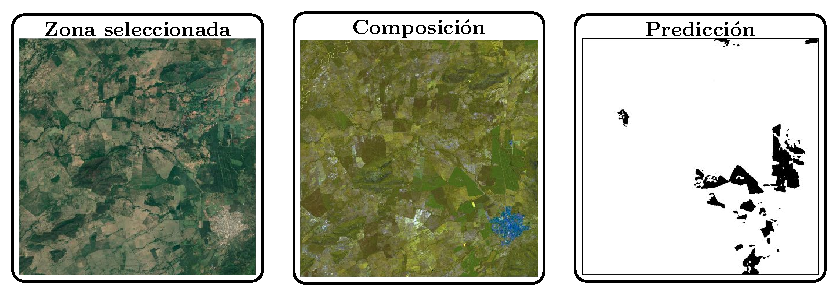
\includegraphics[width=\textwidth]{example_selected_zone}
 \caption{Ejemplo de predicción del modelo sobre un área con cultivos}
 \label{fig:example_selected_zone}
\end{figure*}

En la Figura \ref{fig:example_selected_zone} se muestra una zona seleccionada de 10x10 km en Colombia, seguida de la composición de Sentinel-1 y Sentinel-2. Finalmente, se presenta la salida del modelo, donde la clase 1, representada en negro, indica las áreas clasificadas como palma de aceite, mientras que las zonas en blanco en la máscara corresponden a las áreas donde el modelo identifica que no hay palma de aceite.

\begin{figure*}[t]
 \centering
 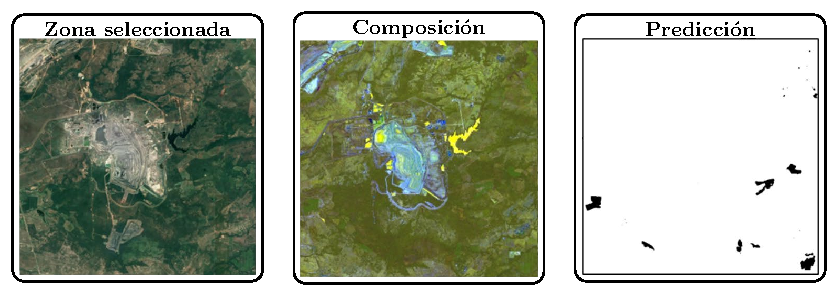
\includegraphics[width=\textwidth]{example_few_crops}
 \caption{Ejemplo de predicción del modelo sobre un área con pocos cultivos}
 \label{fig:example_few_crops}
\end{figure*}

En la Figura \ref{fig:example_few_crops} se observa una zona de explotación minera, que en la composición adquiere un color celeste. También se identifica un cuerpo de agua, representado con un color amarillo en la composición. Por otro lado, las plantaciones de palma de aceite se distinguen por un color verde característico. En esta zona seleccionada, los cultivos de palma de aceite son escasos, lo que explica que el color verde no sea predominante en la imagen. En la máscara predicha por el modelo, se puede apreciar que las áreas con plantaciones de palma de aceite se clasifican correctamente.

\begin{figure*}[t]
 \centering
 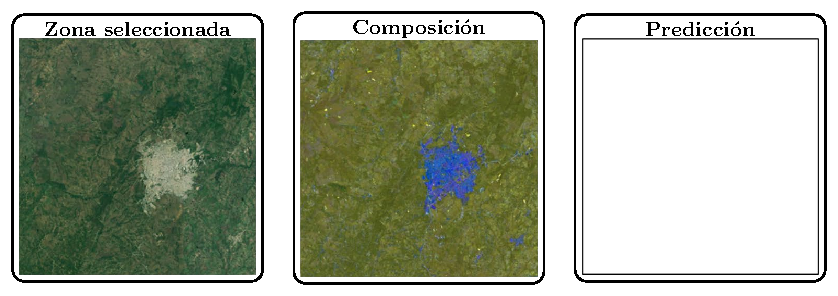
\includegraphics[width=\textwidth]{example_without_crops}
 \caption{Ejemplo de predicción del modelo sobre área sin cultivos}
 \label{fig:example_without_crops}
\end{figure*}

En la Figura \ref{fig:example_without_crops} se muestra una zona seleccionada donde no hay presencia de palma de aceite y, además, se encuentra una área metropolitana. En este caso, se observa que el modelo genera una máscara completamente blanca, lo que indica que clasifica correctamente la ausencia de cultivos de palma de aceite en esta zona.

\begin{figure*}[t]
 \centering
 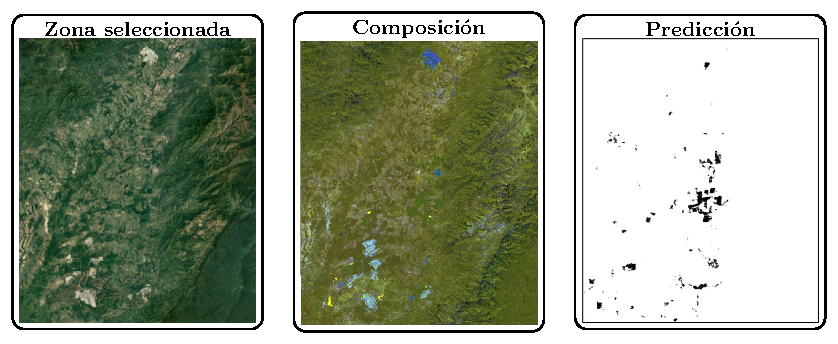
\includegraphics[width=\textwidth]{full_prediction}
 \caption{Predicción del modelo sobre toda la zona seleccionada}
 \label{fig:full_prediction}
\end{figure*}

En la Figura \ref{fig:full_prediction} se presenta la zona seleccionada en su totalidad, que incluye áreas metropolitanas, bosques, diversas plantaciones de otros cultivos, zonas rocosas y una gran diversidad de flora. A continuación, se muestra la predicción, donde las áreas en negro representan las regiones identificadas por el modelo como contenedoras de palma de aceite, mientras que las áreas en blanco indican la ausencia de este cultivo según la clasificación del modelo.

\begin{figure}
 \centering
 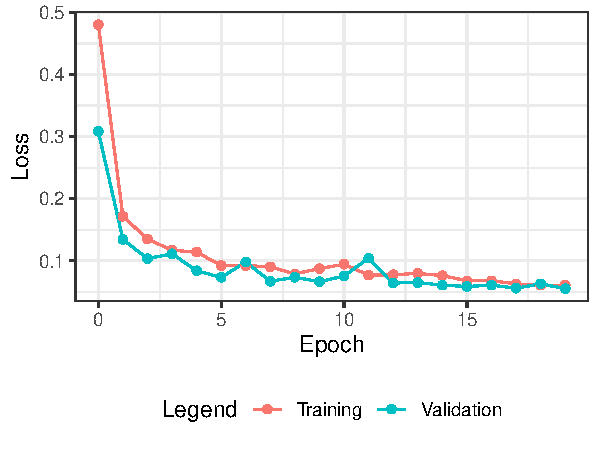
\includegraphics[width=\columnwidth]{loss}
 \caption{Gráfica de perdida (loss)}
 \label{fig:loss}
\end{figure}

\begin{figure}
 \centering
 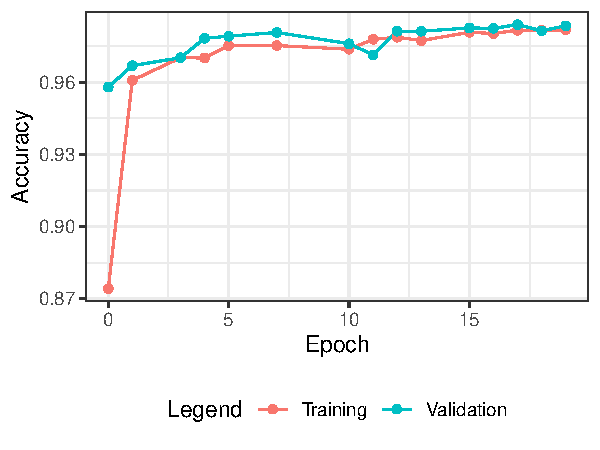
\includegraphics[width=\columnwidth]{accuracy}
 \caption{Gráfica de exactitud (accuracy)}
 \label{fig:accuracy}
\end{figure}

En el gráfico mostrado en la Figura \ref{fig:loss}, se observa la pérdida durante las etapas de  entrenamiento y validación. La pérdida disminuye rápidamente durante las primeras épocas, para luego estabilizarse, lo que sugiere que el modelo alcanzó un punto de convergencia de manera eficiente. De manera similar, en el gráfico \ref{fig:accuracy}, las líneas representan la precisión de entrenamiento y validación, ambas alcanzando valores superiores al 90\% y manteniéndose relativamente constantes después de las primeras épocas, lo que indica un buen ajuste del modelo.

\begin{figure}
 \centering
 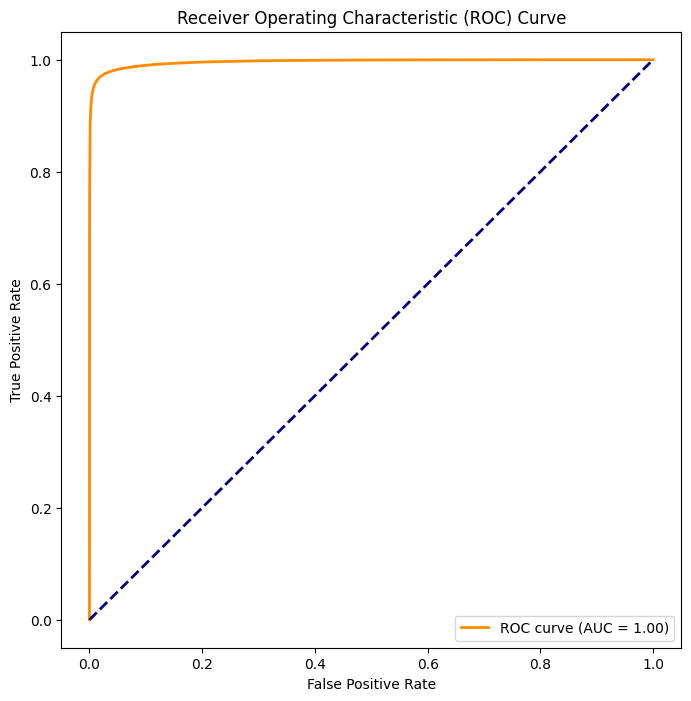
\includegraphics[width=0.8\columnwidth]{roc}
 \caption{Curva ROC del modelo}
 \label{fig:roc}
\end{figure}

La Figura \ref{fig:roc} muestra la Curva Característica de Operación del Receptor (ROC) con un área bajo la curva (AUC) de 1.00. La curva ROC, representada por una línea naranja, se adhiere perfectamente al borde superior izquierdo del gráfico, lo que indica un rendimiento excepcional del modelo. Esto demuestra una tasa de verdaderos positivos del 100\% en todos los umbrales de clasificación, mientras que la tasa de falsos positivos permanece en cero. El gráfico también incluye una línea punteada azul que representa el rendimiento de un clasificador aleatorio, lo que resalta aún más la superioridad del modelo evaluado.

Por último, al comparar este modelo con el presentado por \cite{diaz2023}, se observa que dicho estudio utilizó una variedad de algoritmos de aprendizaje automático más tradicionales, como regresión logística, Random Forest, SVM y XGBoost. Aunque estos métodos son eficaces y versátiles, no son tan específicos como los modelos de Deep Learning para tareas detalladas de segmentación de imágenes. Además, dicho análisis incorporó índices de vegetación y variables de textura, lo que enfatiza aspectos específicos de la vegetación y el terreno. Aunque esta metodología es útil, posiblemente no captura la gama completa de características obtenibles con el enfoque basado en Deep Learning. La precisión del modelo en dicho trabajo fue ligeramente inferior, con un 96\%, lo que sugiere que los enfoques tradicionales de aprendizaje automático siguen siendo efectivos para tareas de clasificación detalladas, aunque menos precisos que los métodos avanzados de Deep Learning.
